\documentclass[12pt]{article}
\usepackage[a4paper,top=35mm,bottom=45mm,left=20mm,right=20mm]{geometry}
\geometry{headheight=16mm,headsep=10mm,footskip=-30mm}

\usepackage[utf8]{inputenc}
\usepackage[portuguese]{babel}
\usepackage{fancyhdr}
\usepackage{array,multirow}
\usepackage[table]{xcolor}
\usepackage{graphicx}
\usepackage{ifthen}

\pagestyle{fancy}
\setlength{\headheight}{4mm}
\setlength\arrayrulewidth{.6pt}

\rhead{
\includegraphics{autobotz}}
\cfoot{
\includegraphics{macro}}
\lhead{\sc \small Equipe de Robótica Autobotz \newline Universidade Federal de Minas Gerais \newline}
\chead{}
\rfoot{}
\lfoot{}

\graphicspath{{report/imagens/}}
\def \semana {41}
\def \dataInicio {9}
\def \dataFim {15 de Outubro de 2017}

\newenvironment{membro}{
	\newcommand{\nome}[1]{\def \nome {##1}}	
	\newcommand{\tarefas}[2]{\def \tarefa {##1} \def \horas {##2}}
	\newcommand{\planos}[1]{\def \plano {##1}}
	\newcommand{\comentarios}[1]{\def \comentario {##1}}
}{
\section*{\nome}~

\textbf{Atividades realizadas nesta semana por \nome:}

\ifthenelse{\horas=0}{~\par\emph{\quad Não preenchido\\}}{ %
\begin{center}
\begin{tabular}%
{| m{.7\textwidth} | >{\centering\arraybackslash}m{3em} |}
\hline
 \rowcolor[RGB]{245,245,245}\centering \bf Atividades & \bf Horas \\
\tarefa
\hline \multicolumn{1}{r|}{Total:} & \cellcolor[RGB]{245,245,245} \bf \horas \\
\cline{2-2}
\end{tabular}
\end{center}
}~

\textbf{Atividades a serem realizadas na próxima semana:}

\ifx\plano\empty~
\par\emph{\quad Não preenchido\\}
\else
\begin{itemize}
\plano
\end{itemize}
\fi~

\textbf{Comentários:}

\ifx\comentario\empty~
\par\emph{\quad Não preenchido\\}
\else
\begin{quote}
\comentario
\end{quote}
\fi
\pagebreak
}

\begin{document}

%\begin{titlepage}
\thispagestyle{fancy}

~\vspace{20mm}

\begin{center}
\textbf{\huge Relatório Semanal de Atividades} \\[8mm]
\textbf{\Large Semana \semana} \\
{\Large \dataInicio\ a \dataFim}
\end{center}

\iffalse
\vfill
\begin{figure}[h]
\centering
Horas por membro

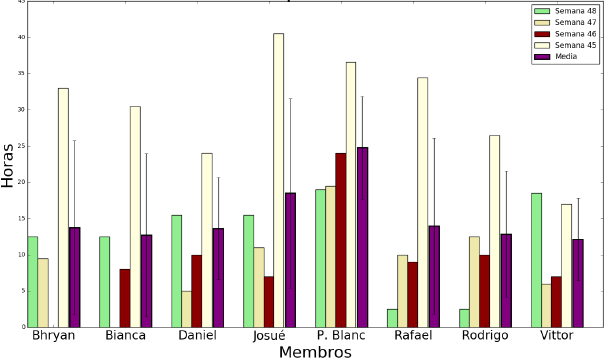
\includegraphics[height=.3\textheight]{grafico_barras}
\end{figure}
\vfill
\begin{figure}[h]
\centering
Porcentagem das horas médias por membro

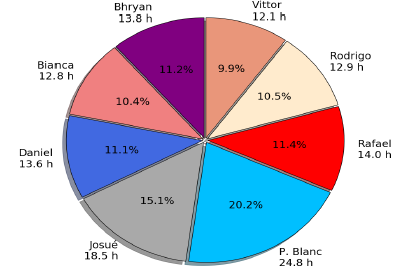
\includegraphics[height=.3\textheight]{grafico_pizza}
\end{figure}
\vfill

\end{titlepage}
\fi

\begin{membro}
\nome{Bárbara Almeida}
\tarefas{\hline apresentação na aula de introdução à engenharia & 1.5 \\
\hline modulo para controle do VT via teclado & 5.75 \\
\hline estudo sobre formas de comunicar Gazebo com rviz & 2.0 \\}{9.25}
\planos{}
\comentarios{}
\end{membro}

\begin{membro}
\nome{Bianca Martins}
\tarefas{}{0}
\planos{}
\comentarios{}
\end{membro}

\begin{membro}
\nome{Bruno Cerqueira}
\tarefas{}{0}
\planos{}
\comentarios{}
\end{membro}

\begin{membro}
\nome{Daniel Leite}
\tarefas{}{0}
\planos{}
\comentarios{}
\end{membro}

\begin{membro}
\nome{Elisa Bacelar}
\tarefas{\hline Estudo da estratégia criada pelos memebros antigos & 3.5 \\
\hline Teste do simulador criado pelos membros antigos & 1.5 \\}{5.0}
\planos{}
\comentarios{}
\end{membro}

\begin{membro}
\nome{Jonatan Campos}
\tarefas{}{0}
\planos{}
\comentarios{}
\end{membro}

\begin{membro}
\nome{Josué Henrique}
\tarefas{}{0}
\planos{}
\comentarios{}
\end{membro}

\begin{membro}
\nome{Mariana Meireles}
\tarefas{\hline trabalhando para a mostra de profissão & 15.0 \\
\hline reunião com o Raffo & 2.5 \\
\hline mostra de prof & 4.0 \\
\hline lidando com bateria e motor, realizando testes, documentando & 2.5 \\
\hline aprendendo Ruby & 2.0 \\
\hline aprendendo Ruby & 4.0 \\}{30.0}
\planos{}
\comentarios{}
\end{membro}

\begin{membro}
\nome{Pedro Blanc}
\tarefas{}{0}
\planos{}
\comentarios{}
\end{membro}

\begin{membro}
\nome{Renan Costa}
\tarefas{}{0}
\planos{}
\comentarios{}
\end{membro}

\begin{membro}
\nome{Rodrigo Cézar}
\tarefas{}{0}
\planos{}
\comentarios{}
\end{membro}

\begin{membro}
\nome{Thiago Lages}
\tarefas{}{0}
\planos{}
\comentarios{}
\end{membro}

\begin{membro}
\nome{Victor Castro}
\tarefas{}{0}
\planos{}
\comentarios{}
\end{membro}



\end{document}